\chapter{Monte Carlo Solution Methods for the Simplified $P_N$ Equations}
\label{ch:spn_equations}

The neutron transport problem is complicated. Solutions cover a large
phase space and the problems of interest are often geometrically
complex, very large, or both, requiring tremendous computational
resources to generate an adequate solution. Modern deterministic
methods for large scale problems are commonly variants on the discrete
ordinates ($S_N$) method \citep{evans_denovo:_2010}. For full reactor
core neutronics simulations, the $S_N$ method requires potentially
trillions of unknown angular flux moments to be computed to achieve
good accuracy for the repsonses of interest
\citep{slaybaugh_acceleration_2011}. Other forms of the transport
problem, including the $P_N$ method, take on a simpler form than the
more common $S_N$ methods but lack in accuracy when compared while
still requiring considerable computational resources for solutions in
multiple dimensions.

In the 1960's, Gelbard developed an ad-hoc multidimensional extension
of the simple single dimension planar $P_N$ equations that created a
system of coupled, diffusion-like equations known as the simplified
$P_N$ ($SP_N$) equations. Up until around the 1990's, the $SP_N$
method was either widely unknown, widely unused, or combination of
both even though numerical studies showed promising results with
better solutions than diffusion theory and a significant reduction in
computational time over more accurate methods such as discrete
ordinates. Why did this happen? A significant problem, pointed out by
Brantley and Larsen \citep{brantley_simplified_2000}, was that little
rigor had been applied to the formulation of the $SP_N$ equations
since their derivation through primarily heuristic arguments. Instead,
studies at that time focused on simply comparing the results of the
method to other contemporary transport solution strategies. In
addition, many problems of interest from the literature at the time
were either solved using nodal-type methods for reactor-sized problems
or $S_N$-type methods for benchmark problems with intricate material
configurations and potentially large flux gradients over small spatial
domains.

So why reconsider the $SP_N$ equations? Starting in the 1990's and
primarily due to Larsen and his colleagues, the $SP_N$ equations have
been given a more rigorous treatment with both variational and
asymptotic derivations performed as a means of verification. In
addition, these equations have been more rigorously studied as
solution methods to MOX fuel problems and have been shown to provide
accurate solutions. With this mathematical literature to provide a
solid numerical footing for the method, we look at its application to
today's challenge problems in full reactor core transport. The
reduction in numerical complexity of current full core deterministic
solution methods using the $S_N$ approximation could mean significant
savings in both compute time and memory required. In addition, the
characteristics of the solution to the transport problem for a steady
state reactor core permit diffusion theory to be used; a staple of the
nuclear industry since its inception. Therefore, if diffusion theory
is applicable, then finer grained solutions that capture more of the
physics contained in the transport equation should be possible with
the $SP_N$ method. In doing so, we also expect from the literature to
obtain computed responses on the order of accuracy we would expect
from an appropriately discretized $S_N$ method at a fraction of the
cost. 

To further motivate moving in this direction, recent developments in
the Exnihilo neutronics package at Oak Ridge National Laboratory have
permitted generation of the $SP_N$ system of equations for detailed
full core reactor models \citep{evans_simpli_2013}. By fully forming
these equations and formulating them as a linear algebra problem
instead of using the explicit iterative methods of the past, we now
have access to all of the modern advancements in computational linear
algebra including Krylov solvers for asymmetric systems and
preconditioning methods such as algebraic multigrid. This leads us to
then explore the applicability of our work in discrete Monte Carlo
methods for linear systems as a possible solution method for the
$SP_N$ equations. If formulated correctly, we hypothesize that
significant improvement in usage of computational resources may be
observed compared to modern solution techniques such as those
suggested due to the form of the matrices generated by the
discretization. In addition, solving the $SP_N$ equations in this way
also breaks away from the $S_N$ forms of parallelism where spatial
parallelism is achieved by an efficient parallel sweep, angular
efficiency achieved by pipelining, and energy parallelism achieved by
decoupling the groups. With the $SP_N$ equations as a full matrix
system, we now can parallelize the problem as prescribed by the linear
solver, which may be significantly more scalable than current $S_N$
transport practices.

In this chapter, we derive the $SP_N$ equations, closely following the
work of Evans\footnote{The $SP_N$ derivations in this chapter are
  heavily based on those presented by Evans in
  \citep{evans_simpli_2013}}, in order to gain full understanding of
the underlying system and its potential behavior in a Monte Carlo
context. From the $P_N$ equations, we apply a set of approximations to
yield the multi-dimensional, multi-group $SP_N$ equations for fixed
source problems. Using the fully-formed matrix for the transport
problem, we explore solutions to the $SP_N$ equations using Monte
Carlo Synthetic Acceleration using a light water reactor fuel assembly
criticality calculation as the driving problem.

%%---------------------------------------------------------------------------%%
\section{The Neutron Transport Equation}
\label{sec:transport_eq}
As a starting point we define the time-independent neutron transport
equation \citep{lewis_computational_1993}:
\begin{multline}
  \hat{\Omega} \cdot \vec{\nabla} \psi(\vec{r},\hat{\Omega},E) +
  \sigma(\vec{r},E) \psi(\vec{r},\hat{\Omega},E) = \\ \iint
  \sigma_s(\vec{r},E' \rightarrow E,\hat{\Omega}' \cdot \hat{\Omega})
  \psi(\vec{r},\hat{\Omega}',E') d\Omega' dE' +
  q(\vec{r},\hat{\Omega},E)\:,
  \label{eq:general_transport}
\end{multline}
with the variables defined as:
\begin{itemize}
\item $\vec{r}$ - neutron spatial position
\item $\hat{\Omega}$ - neutron streaming direction with radial
  component $\mu$ and azimuthal component $\omega$
\item $\hat{\Omega}' \cdot \hat{\Omega} = \mu_0$ is the angle of
  scattering
\item $E$ - neutron energy
\item $\psi(\vec{r},\hat{\Omega},E)$ - angular flux
\item $\sigma(\vec{r},E)$ - total interaction cross section
\item $\sigma_s(\vec{r},E' \rightarrow E,\hat{\Omega}')$ - probability
  of scattering from direction $\hat{\Omega}'$ into an angular domain
  $d\hat{\Omega}'$ about the direction $\hat{\Omega}$ and from energy
  $E'$ to an energy domain $dE'$ about energy $E$
\item $q(\vec{r},\hat{\Omega},E)$ - external source of neutrons.
\end{itemize}
For this work, it is sufficient to formulate
Eq~(\ref{eq:general_transport}) in 1-dimensonal Cartesian geometry:
\begin{multline}
  \mu \frac{\partial}{\partial x} \psi(x,\mu,E) + \sigma(x,E)
  \psi(x,\mu,E) = \\ \iint \sigma_s(x,E' \rightarrow E,\hat{\Omega}'
  \cdot \hat{\Omega}) \psi(x,\hat{\Omega}',E') d\Omega' dE' +
  \frac{q(x,E)}{4 \pi}\:,
  \label{eq:cart_1d_transport}
\end{multline}
where the angular component of the solution is no longer dependent on
the azimuthal direction of travel and an isotropic source of neutrons
is assumed. In addition, for fission systems the eigenvalue form of the transport
equation is:
\begin{multline}
  \hat{\Omega} \cdot \vec{\nabla} \psi(\vec{r},\hat{\Omega},E) +
  \sigma(\vec{r},E) \psi(\vec{r},\hat{\Omega},E) = \\ \iint
  \sigma_s(\vec{r},E' \rightarrow E,\hat{\Omega}' \cdot \hat{\Omega})
  \psi(\vec{r},\hat{\Omega}',E') d\Omega' dE' + \\ \frac{1}{k} \chi(E)
  \iint \nu \sigma_f(\hat{r},E') \psi(\vec{r},\hat{\Omega}',E')
  d\Omega' dE' + q(\vec{r},\hat{\Omega},E) \:,
  \label{eq:eigenvalue_transport}
\end{multline}
with the additional variables defined as
\begin{itemize}
\item $k$ - multiplication factor
\item $\chi(E)$ - fission neutron energy spectrum
\item $\nu$ - average number of neutrons per fission
\item $\sigma_f(r,E')$ - fission cross section\:.
\end{itemize}
In 1-dimensional cartesian geometry,
Eq~(\ref{eq:eigenvalue_transport}) becomes:
\begin{multline}
  \mu \frac{\partial}{\partial x} \psi(x,\mu,E) + \sigma(x,E)
  \psi(x,\mu,E) = \\ \iint \sigma_s(x,E' \rightarrow
  E,\hat{\Omega}' \cdot \hat{\Omega}) \psi(x,\hat{\Omega}',E')
  d\Omega' dE' + \\ \frac{1}{k} \chi(E)
  \iint \nu \sigma_f(x,E') \psi(x,\hat{\Omega}',E') d\Omega'
  dE' + \frac{q(x,E)}{4 \pi}\:.
  \label{eq:cart_1d_eigenvalue}
\end{multline}

%%---------------------------------------------------------------------------%%
\section{Derivation of the Monoenergetic $SP_N$ Equations}
\label{sec:spn_equations}
The $P_N$ equations as derived in Appendix~\ref{chap:pn_equations}
give $N+1$ coupled first-order equations capturing the spatial and
angular-dependence of the solution. In multiple dimensions, the
equation set becomes large and coupled not only through angular
moments but also through the spatial variables. As a simpler
alternative to multidimensional $P_N$ solutions, Gelbard recognized in
1960 that the planar $P_N$ equations could be simplified and applied
an ad-hoc method to extend them to multiple dimensions, yielding the
$SP_N$ equations. These equations are not only fewer in number, but
also take on a diffusion-like form while maintaining the angular
character of the flux, making them amenable to solutions with modern
diffusion methods.

First, the $P_N$ equations can be simplified to $(N+1)/2$ second-order
equations by solving for the $n^{th}$ Legendre flux moment in the
odd-order equations:
\begin{equation}
  \phi_n = \frac{1}{\Sigma_n}\Bigg[ q \delta_{no} -
    \frac{\partial}{\partial x}\Big(\frac{n}{2n+1}\phi_{n-1} +
    \frac{n+1}{2n+1} \phi_{n+1} \Big) \Bigg]\:, 
  \label{eq:odd_moments}
\end{equation}
for $n = 1,3,\cdots,N$ and $\delta_{no} = 0\ \forall n \neq 0$. We can
insert the odd moments into Eq~(\ref{eq:final_pn_equations}) to get a
reduced group of equations for the even moments:
\begin{multline}
  -\frac{\partial}{\partial x}
  \Bigg[\frac{n}{2n+1}\frac{1}{\Sigma_{n-1}} \frac{\partial}{\partial
      x} \Big(\frac{n-1}{2n-1} \phi_{n-2} + \frac{n}{2n-1}\phi_n \Big)
    \\+ \frac{n+1}{2n+1}\frac{1}{\Sigma_{n+1}} \frac{\partial}{\partial
      x} \Big(\frac{n+1}{2n+3}\phi_n + \frac{n+2}{2n+3}\phi_{n+2}\Big)
    \Bigg] \\+ \Sigma_n \phi_n = q \delta_{n0}\ \ \ \ \ \ \ \ \ n =
  0,2,4,\cdots,N\:.
  \label{eq:reduced_pn}
\end{multline}
Immediately, we note the diffusion-like nature of
Eq~(\ref{eq:reduced_pn}) as compared to the original $P_N$
equations. To extend these equations to multiple dimensions, Gelbard
simply replaced the planar spatial derivatives in the reduced set of
equations with general multidimensional gradient operators:
\begin{multline}
  -\nabla \cdot \Bigg[\frac{n}{2n+1}\frac{1}{\Sigma_{n-1}} \nabla
    \Big(\frac{n-1}{2n-1} \phi_{n-2} + \frac{n}{2n-1}\phi_n \Big) \\+
    \frac{n+1}{2n+1}\frac{1}{\Sigma_{n+1}} \nabla
    \Big(\frac{n+1}{2n+3}\phi_n + \frac{n+2}{2n+3}\phi_{n+2}\Big)
    \Bigg] \\+ \Sigma_n \phi_n = q \delta_{n0}\ \ \ \ \ \ \ \ \ n =
  0,2,4,\cdots,N\:,
  \label{eq:spn_equations}
\end{multline}
yielding a multidimensional set of $(N+1)/1$ angular coupled equations
defined as the $SP_N$ equations. As with the $P_N$ equations, we
provide closure to this set of equations with $\phi_{N+1} = 0$. As a
concrete example, we will consider the $SP_7$ equations:
\begin{subequations}
  \begin{gather}
    -\nabla \cdot \frac{1}{3 \Sigma_1} \nabla ( \phi_0 + 2\phi_2 ) +
    \Sigma_0 \phi_0 = q \\ 
    -\nabla \cdot \Bigg[ \frac{2}{15 \Sigma_1} \nabla ( \phi_0 + 2\phi_2
      ) + \frac{3}{35 \Sigma_3}\nabla( 3\phi_2 + 4\phi_4)\Bigg] +
    \Sigma_2 \phi_2 = 0\\
    -\nabla \cdot \Bigg[ \frac{4}{63 \Sigma_3} \nabla ( 3\phi_2 +
      4\phi_4 ) + \frac{5}{99 \Sigma_5}\nabla( 5\phi_4 +
      6\phi_6)\Bigg] + \Sigma_4 \phi_4 = 0\\
    -\nabla \cdot \Bigg[ \frac{6}{143 \Sigma_5} \nabla ( 5\phi_4 +
      6\phi_6 ) + \frac{7}{195 \Sigma_7}\nabla(7\phi_6)\Bigg] +
    \Sigma_6 \phi_6 = 0 \:.
  \end{gather}
  \label{eq:sp7_equations}
\end{subequations}
To further modify these equations, we can use a change of variables to
create a new group of equations such that the gradients are operating
on a single vector:
\begin{subequations}
  \begin{gather}
    u_1 = \phi_0 + 2\phi_2 \\
    u_2 = 3\phi_2 + 4\phi_4 \\
    u_3 = 5\phi_4 + 6\phi_6 \\
    u_4 = 7\phi_6 \:,
  \end{gather}
  \label{eq:spn7_subs}
\end{subequations}
or equivalently:
\begin{subequations}
  \begin{gather}
    \phi_0 = u_1 - \frac{2}{3}u_2 + \frac{8}{15}u_3 -
    \frac{16}{35}u_4 \\
    \phi_2 = \frac{1}{3}u_2 - \frac{4}{15}u_3 + \frac{8}{35}u_4\\ 
    \phi_4 = \frac{1}{5}u_3 - \frac{6}{35}u_4\\
    \phi_6 = \frac{1}{7}u_4\:.
  \end{gather}
  \label{eq:spn7_subs_inverse}
\end{subequations}
When substituted into Eq~(\ref{eq:sp7_equations}), these terms give:
\begin{subequations}
  \begin{gather}
    -\nabla \cdot \frac{1}{3 \Sigma_1} \nabla u_1 + \Sigma_0 \Bigg[
    u_1 - \frac{2}{3}u_2 + \frac{8}{15}u_3 - \frac{16}{35}u_4 \Bigg]
    = -q \\
    -\nabla \cdot \Bigg[ \frac{2}{15 \Sigma_1} \nabla u_1 +
    \frac{3}{35 \Sigma_3} \nabla u_2 \Bigg] + \Sigma_2 \Bigg[
    \frac{1}{3}u_2 - \frac{4}{15}u_3 + \frac{8}{35}u_4 \Bigg] = 0 \\
    -\nabla \cdot \Bigg[ \frac{4}{63 \Sigma_3} \nabla u_2 +
    \frac{5}{99 \Sigma_5} \nabla u_3 \Bigg] + \Sigma_4 \Bigg[
    \frac{1}{5}u_3 - \frac{6}{35}u_4 \Bigg] = 0 \\ 
    -\nabla \cdot \Bigg[ \frac{6}{143 \Sigma_5} \nabla u_3 +
    \frac{7}{195 \Sigma_7} \nabla u_4 \Bigg] + \Sigma_6 \Bigg[
    \frac{1}{7}u_4 \Bigg] = 0 \:.
  \end{gather}
  \label{eq:spn7_subs_equations}
\end{subequations}
If we rearrange Eq~(\ref{eq:spn7_subs_equations}) such that only one
divergence operation is present in each equation, we can formulate
this as a matrix system of 4 equations in the case of the $SP_7$
approximation:
\begin{equation}
  -\nabla \cdot D_n \nabla u_n + \sum_{m=1}^4 A_{nm} u_m =
  q_n\ \ \ \ \ \ \ n = 1,2,3,4\:,
  \label{eq:spn_matrix}
\end{equation}
with $\mathbf{u}$ the vector of solution variables:
\begin{equation}
  \mathbf{u} = ( u_1\ \ u_2\ \ u_3\ \ u_4 )^T \:,
  \label{eq:spn7_solution_vector}
\end{equation}
$\mathbf{D}$ the vector of effective diffusion coefficients:
\begin{equation}
  \mathbf{D} = \Bigg( \frac{1}{3\Sigma_1}\ \ \frac{1}{7\Sigma_3}\ \
  \frac{1}{11\Sigma_5}\ \ \frac{1}{15\Sigma_7} \Bigg)^T\:,
  \label{eq:spn7_diffusion_coeffs}
\end{equation}
$\mathbf{q}$ the vector of source terms where the $0^{th}$ moment
source has now been distributed through the system:
\begin{equation}
  \mathbf{q} = (
  q\ \ -\frac{2}{3}q\ \ \frac{8}{15}q\ \ -\frac{16}{35}q )^T\:,
  \label{eq:spn7_source_vector}
\end{equation}
and $\mathbf{A}$ a matrix of angular scattering terms:
% NOTE: I copied the following matrix directly out of Tom's tech note
% on the SPn equations which I am effectively following here because I
% was feeling lazy. I have verified its correctness.
\begin{equation}
  \mathbf{A} = 
  {\tiny \begin{bmatrix}
    (\Sigma_0) &
    (-\frac{2}{3}\Sigma_0) &
    (\frac{8}{15}\Sigma_0) &
    (-\frac{16}{35}\Sigma_0) \\
    %%
    &&&\\
    %%
    (-\frac{2}{3}\Sigma_0) &
    (\frac{4}{9}\Sigma_0 + \frac{5}{9}\Sigma_2) &
    (-\frac{16}{45}\Sigma_0 - \frac{4}{9}\Sigma_2) &
    (\frac{32}{105}\Sigma_0 + \frac{8}{21}\Sigma_2) \\
    %%
    &&&\\
    %%
    (\frac{8}{15}\Sigma_0) &
    (-\frac{16}{45}\Sigma_0 - \frac{4}{9}\Sigma_2) &
    (\frac{64}{225}\Sigma_0 + \frac{16}{45}\Sigma_2 + \frac{9}{25}\Sigma_4) &
    (-\frac{128}{525}\Sigma_0 - \frac{32}{105}\Sigma_2 - \frac{54}{175}\Sigma_4)
    \\ 
    %%
    &&&\\
    %%
    (-\frac{16}{35}\Sigma_0) &
    (\frac{32}{105}\Sigma_0 + \frac{8}{21}\Sigma_2) &
    (-\frac{128}{525}\Sigma_0 - \frac{32}{105}\Sigma_2 - \frac{54}{175}\Sigma_4)
    & 
    (\frac{256}{1225}\Sigma_0 + \frac{64}{245}\Sigma_2 +
    \frac{324}{1225}\Sigma_4 + \frac{13}{49}\Sigma_6)
  \end{bmatrix}}\:.
  \label{eq:A_matrix}
\end{equation}
Note that the term $\sum_{m=1}^4 A_{nm} u_m$ in
Eq~(\ref{eq:spn_matrix}) couples the moments in each equation while
the diffusive term in each equation is only for a single
'psuedo-moment' $u_n$. As noted by Evans \citep{evans_simpli_2013},
lower order $SP_N$ approximations can be generated by setting higher
order even moments in this system to zero (e.g. $\phi_6 = \phi_4 = 0$
yields the $SP_3$ equations). Boundary conditions for these equations
are provided in Appendix~\ref{chap:spn_boundary_conditions}.

%%---------------------------------------------------------------------------%%
\section{Derivation of the Multigroup $SP_N$ Equations}
\label{sec:mg_spn_equations}
Up to this point, we have formulated the $SP_N$ equations for a single
neutron energy. To expand these equations for multiple energies, we
start by stating the multigroup neutron transport equation for a
single dimension in planar geometry:
\begin{multline}
  \mu \frac{\partial}{\partial x} \psi^g(x,\mu) + \sigma^g(x)
  \psi^g(x,\mu) = \\ \sum_{g'=0}^{G} \int
  \sigma_s^{gg'}(x,\hat{\Omega}' \rightarrow \hat{\Omega})
  \psi^{g'}(x,\hat{\Omega}') d\Omega' + \frac{q^g(x)}{4 \pi}\:,
  \label{eq:cart_1d_multigroup}
\end{multline}
where $g$ denotes the group index of $0$ to $G$ groups, $G=N_g-1$, and
the integration of the scattering emission term over energy has been
replaced by a discrete summation. For scattering, $\sigma_s^{gg'}$
provides the probability of scattering at a particular angle from
group $g$ to $g'$. The result is an equation nearly identical in form
to Eq~(\ref{eq:cart_1d_transport}) where now instead of forming the
$SP_N$ equations for a single energy group, we form them for each of
the energy groups with group coupling occuring through the scattering
term. The multigroup $P_N$ equations are then:
\begin{equation}
   \frac{1}{2n+1} \frac{\partial}{\partial x}\Big[ (n+1) \phi^g_{n+1}
     + n \phi^g_{n-1} \Big] +
   \sum_{g'}(\sigma^g\delta_{gg'}-\sigma^{gg'}_{sn}) \phi^g_n =
   q\delta_{n0} \:,
  \label{eq:multigroup_pn_equations}
\end{equation}
for $n = 0,1,\dotsc,N$ where the flux and scattering moments are
defined in a group. We observe that a $N_g \times N_g$ scattering
matrix is formed:
\begin{equation}
  \mathbf{\Sigma}_n =
  \sum_{g'}(\sigma^g\delta_{gg'}-\sigma^{gg'}_{sn})\:,
  \label{eq:scattering_matrix}
\end{equation}
and when expanded gives:
%% Also grabbed this matrix from Tom's tech note.
\begin{equation}
  \mathbf{\Sigma}_n =
  \begin{bmatrix}
    (\sigma^0-\sigma_{sn}^{00}) & -\sigma_{sn}^{01} & \dots &
    -\sigma_{sn}^{0G} \\ &&&\\ -\sigma_{sn}^{10} &
    (\sigma^1-\sigma_{sn}^{11}) & \dots & -\sigma_{sn}^{1G}
    \\ &&&\\ \vdots & \vdots & \ddots & \vdots
    \\ &&&\\ -\sigma_{sn}^{G0} & -\sigma_{sn}^{G1} & \dots &
    (\sigma^G-\sigma_{sn}^{GG})
  \end{bmatrix}\:.
\end{equation}
It is also useful to combine the group flux moments and sources into a
single vector for more compact notation:
\begin{equation}
  \mathbf{\Phi_n} = (\phi^0_n\ \phi^1_n\ \cdots \phi^G_n )^T\:, 
  \label{eq:group_flux_vector}
\end{equation}
\begin{equation}
  \mathbf{q} = (q^0\ q^1\ \cdots q^G )^T\:.
  \label{eq:group_source_vector}
\end{equation}
Next, we apply the $SP_N$ approximation to
Eq~(\ref{eq:multigroup_pn_equations}) in identical fashion to the
monoenergetic case. This gives:
\begin{multline}
  -\nabla \cdot \Bigg[\frac{n}{2n+1}\mathbf{\Sigma_{n-1}}^{-1} \nabla
    \Big(\frac{n-1}{2n-1} \mathbf{\Phi_{n-2}} +
    \frac{n}{2n-1}\mathbf{\Phi_n} \Big) \\+
    \frac{n+1}{2n+1}\mathbf{\Sigma_{n+1}}^{-1} \nabla
    \Big(\frac{n+1}{2n+3}\mathbf{\Phi_n} +
    \frac{n+2}{2n+3}\mathbf{\Phi_{n+2}}\Big) \Bigg] \\+
  \mathbf{\Sigma_n} \mathbf{\Phi_n} = \mathbf{q}
  \delta_{n0}\ \ \ \ \ \ \ \ \ n = 0,2,4,\cdots,N\:.
  \label{eq:multigroup_spn_equations}
\end{multline}
This adds more complexity than the monoenergetic formulation in that
all unknowns in this group of equations are now vector quantities and
scattering relationships are contained in matrices rather than a
scalar quantity. Because of this, the same sequence of variable
changes and algebra can be used to build a set of matrix equations,
this time in a block formulation:
\begin{equation}
  -\nabla \cdot \mathbb{D}_n \nabla \mathbb{U}_n + \sum_{m=1}^4
  \mathbb{A}_{nm} \mathbb{U}_m = \mathbb{Q}_n\:,
  \label{eq:spn_multigroup_system}
\end{equation}
where the definition of all quantities are the same with internal
scalar values replaced by the group-vector values. In addition,
$\mathbb{A}$ is now a block matrix of $N_g \times N_g$ submatrices
generated from the moment scattering matrices:
\begin{equation}
  \mathbf{A} = 
  {\tiny \begin{bmatrix}
    (\mathbf{\Sigma}_0) &
    (-\frac{2}{3}\mathbf{\Sigma}_0) &
    (\frac{8}{15}\mathbf{\Sigma}_0) &
    (-\frac{16}{35}\mathbf{\Sigma}_0) \\
    %%
    &&&\\
    %%
    (-\frac{2}{3}\mathbf{\Sigma}_0) &
    (\frac{4}{9}\mathbf{\Sigma}_0 + \frac{5}{9}\mathbf{\Sigma}_2) &
    (-\frac{16}{45}\mathbf{\Sigma}_0 - \frac{4}{9}\mathbf{\Sigma}_2) &
    (\frac{32}{105}\mathbf{\Sigma}_0 + \frac{8}{21}\mathbf{\Sigma}_2) \\
    %%
    &&&\\
    %%
    (\frac{8}{15}\mathbf{\Sigma}_0) &
    (-\frac{16}{45}\mathbf{\Sigma}_0 - \frac{4}{9}\mathbf{\Sigma}_2) &
    (\frac{64}{225}\mathbf{\Sigma}_0 + \frac{16}{45}\mathbf{\Sigma}_2 + \frac{9}{25}\mathbf{\Sigma}_4) &
    (-\frac{128}{525}\mathbf{\Sigma}_0 - \frac{32}{105}\mathbf{\Sigma}_2 - \frac{54}{175}\mathbf{\Sigma}_4)
    \\ 
    %%
    &&&\\
    %%
    (-\frac{16}{35}\mathbf{\Sigma}_0) &
    (\frac{32}{105}\mathbf{\Sigma}_0 + \frac{8}{21}\mathbf{\Sigma}_2) &
    (-\frac{128}{525}\mathbf{\Sigma}_0 - \frac{32}{105}\mathbf{\Sigma}_2 - \frac{54}{175}\mathbf{\Sigma}_4)
    & 
    (\frac{256}{1225}\mathbf{\Sigma}_0 + \frac{64}{245}\mathbf{\Sigma}_2 +
    \frac{324}{1225}\mathbf{\Sigma}_4 + \frac{13}{49}\mathbf{\Sigma}_6)
  \end{bmatrix}}\:.
  \label{eq:A_block_matrix}
\end{equation}
Boundary conditions for these equations are provided in
Appendix~\ref{chap:spn_boundary_conditions}.

\subsection{Spatial Discretization of the $SP_N$ Equations}
\label{subsec:spatial_discretization}
To this point, the formulation of the multigroup $SP_N$ equations
presented have discretized the transport equation in angle and energy
but have yet to consider the spatial component of phase space. Of
primary interest here is the discretization of the diffusive term in
Eq~(\ref{eq:spn_multigroup_system}) and the current term on the
boundaries in Eq~(\ref{eq:spn_multigroup_bnd}). Many popular choices
for spatial discretization are available here and include finite
difference and finite element formulations. In the Exnihilo package at
ORNL, Evans has implemented a finite volume scheme over a Cartesian
grid for these equations resulting in:
\begin{multline}
  - \mathbb{C}_{n,i+1} \mathbb{U}_{n_i+1} - \mathbb{C}_{n,i-1}
  \mathbb{U}_{n_i-1} - \mathbb{C}_{n,j+1} \mathbb{U}_{n_j+1} -
  \mathbb{C}_{n,j-1} \mathbb{U}_{n_j-1} - \mathbb{C}_{n,k+1}
  \mathbb{U}_{n_k+1} - \mathbb{C}_{n,k-1} \mathbb{U}_{n_k-1}
  +\\ \sum_{m=1}^4 \Big[\mathbb{A}_{nm,ijk} +
    (\mathbb{C}_{n,i+1}+\mathbb{C}_{n,j+1}+\mathbb{C}_{n,k+1}+
    \mathbb{C}_{n,i-1}+\mathbb{C}_{n,j-1}+\mathbb{C}_{n,k-1})\delta_{nm}\Big]
  \mathbb{U}_{m,ijk} = \mathbb{Q}_{n,ijk}\:,
  \label{eq:spn_space}
\end{multline}
with the coefficients defined as:
\begin{equation}
  \mathbb{C}_{n,l+1} = \frac{2}{\Delta_l}\Bigg( \frac{\mathbb{D}_{n,l+1}
    \mathbb{D}_{n,l}}{\Delta_l \mathbb{D}_{n,l+1} + \Delta_{l+1} \mathbb{D}_{n,l}}\Bigg)\:,
  \label{eq:spn_coeff_plus}
\end{equation}
\begin{equation}
  \mathbb{C}_{n,l-1} = \frac{2}{\Delta_l}\Bigg( \frac{\mathbb{D}_{n,l}
    \mathbb{D}_{n,l-1}}{\Delta_{l-1} \mathbb{D}_{n,l} + \Delta_{l}
    \mathbb{D}_{n,l-1}}\Bigg)\:,
  \label{eq:spn_coeff_minus}
\end{equation}
where $l={i,j,k}$ along the cardinal directions of the Cartesian grid
cell in Figure~\ref{fig:mesh_cell}. The details of the derivation are
provided in Appendix~\ref{chap:spn_spatial_discretization}.

Although arbitrary grids could be handled effectively
through a finite element scheme, the rectilinear grid used in Denovo
is easily discretized through the finite volume method in a
conservative form. This conservative form is ideal for the
diffusion-like equations in the domain given by
Eq~(\ref{eq:spn_multigroup_system}) and the effective boundary current
conditions given by Eq~(\ref{eq:spn_multigroup_bnd}) as the neutron
current is balanced from cell-to-cell, continuity of the flux is
preserved across cell/material boundaries, and boundary conditions are
naturally represented through cell-face currents. Furthermore, this
spatial discretization is a natural extension of the balance
principles used to arrive at the general transport equation.

\subsection{Eigenvalue Form of the $SP_N$ Equations}
\label{subsec:eigenvalue_form}
For criticality problems, the space, angle, and energy discretizations
for the $SP_N$ equations can be applied to the general eigenvalue from
of the transport equation given by
Eq~(\ref{eq:eigenvalue_transport}). We can readily replace the fixed
source in Eq~(\ref{eq:multigroup_spn_equations}) with the fission
source derived in \S~\ref{sec:pn_eigenvalue}:
\begin{multline}
  -\nabla \cdot \Bigg[\frac{n}{2n+1}\mathbf{\Sigma_{n-1}}^{-1} \nabla
    \Big(\frac{n-1}{2n-1} \mathbf{\Phi_{n-2}} +
    \frac{n}{2n-1}\mathbf{\Phi_n} \Big) \\+
    \frac{n+1}{2n+1}\mathbf{\Sigma_{n+1}}^{-1} \nabla
    \Big(\frac{n+1}{2n+3}\mathbf{\Phi_n} +
    \frac{n+2}{2n+3}\mathbf{\Phi_{n+2}}\Big) \Bigg] \\+
  \mathbf{\Sigma_n} \mathbf{\Phi_n} = \frac{1}{k} \mathbf{F}
  \mathbf{\Phi_n} \delta_{n0} \ \ \ \ \ \ \ \ \ n = 0,2,4,\cdots,N\:.
  \label{eq:multigroup_spn_eigenvalue}
\end{multline}
with the fission matrix $\mathbf{F}$ given by
Eq~(\ref{eq:fission_matrix}). We again apply the change of variables
to yield the set of pseudo-moments $\mathbb{U}_n$ where now the
application of the fission matrix to the moment vectors will be
expanded into a set of block matrices in identical fashion to the
scattering matrices.

It should be noted here that with respect to a general MCSA scheme,
the introduction of the fission in the system will only affect the
source vector in the linear system. The linear operator, and therefore
overall MCSA performance will be dictated by streaming and scattering
as defined on the left-hand side.

%%---------------------------------------------------------------------------%%
\section{Spectral Analysis of the $SP_N$ Equations}
\label{sec:spn_spectral_analysis}
Before we can move on to solving the $SP_N$ equations with both
conventional and Monte Carlo methods, we must first understand their
spectral character to ensure that MCSA will be applicable. As
presented in Chapter~\ref{ch:stochastic_methods}, the spectral radius
of the iteration matrix must be less than unity to ensure
convergence. Therefore, we will compute the spectral radius of the
iteration matrix formed by the $SP_N$ equations while parametrically
varying the $SP_N$ order, the $P_N$ order, the number of energy
groups, and upscattering/downscattering between energy groups. For
each problem in the parameter study, the values given in
Table~\ref{tab:spn_fixed_parameters} were fixed for each spatial
location and energy group.
\begin{table}[h!]
  \begin{center}
    \begin{tabular}{ll}\hline\hline
      \multicolumn{1}{c}{Parameter}& 
      \multicolumn{1}{c}{Value} \\\hline
      Mesh Element Size & 1.0 \\
      Mesh Elements & $4 \times 4 \times 4$ \\
      Reflecting Boundaries & True \\
      Materials & 1 \\
      Source Strength & 1.0 \\
      Total Cross Section & 5.0 \\
      In-Group Cross Section & 0.25 \\
      Downscatter Cross Section & 1.0 \\
      Upscatter Cross Section & 0.1 \\
      Eigenvalue Solver Tolerance & $1.0\times10^{-8}$ \\
      %%
      \hline\hline
    \end{tabular}
  \end{center}
  \caption{\textbf{Fixed parameters for the $SP_N$ spectral radius
      parameter study.} \textit{The parameters were fixed for each
      spatial location and energy group.}}
  \label{tab:spn_fixed_parameters}
\end{table}
Mesh element sizes were the same in all cardinal directions with
reflecting conditions on each boundary. For the energy parameter, 1
and 10 energy groups were used with upscatter/downscatter varied for
the 10 group case. For the downscatter cases, all groups could scatter
to all lower energy groups with the cross sections given in
Table~\ref{tab:spn_fixed_parameters} while for the upscatter case all
groups could scatter to all other energy groups with different cross
sections for upscatter and downscatter used. A uniform isotropic
source of neutrons is given in each group as well.

The matrices generated by the discretization of this problem are
sparse with a block-based form as dictated by
Eq~(\ref{eq:spn_multigroup_system}). Figure~\ref{fig:group1} gives the
sparsity pattern for a monoenergetic $SP_7$ discretization while
Figures~\ref{fig:group10ds} and \ref{fig:group10us} give the sparsity
patterns for the same problem for 10 energy groups without and with
upscatter respectively. For these figures, the parameters in
Table~\ref{tab:spn_fixed_parameters} with the number of spatial
elements reduced to $2 \times 2 \times 2$ to show the blocks generated
by the discretization.
\begin{figure}[t!]
  \begin{center}
    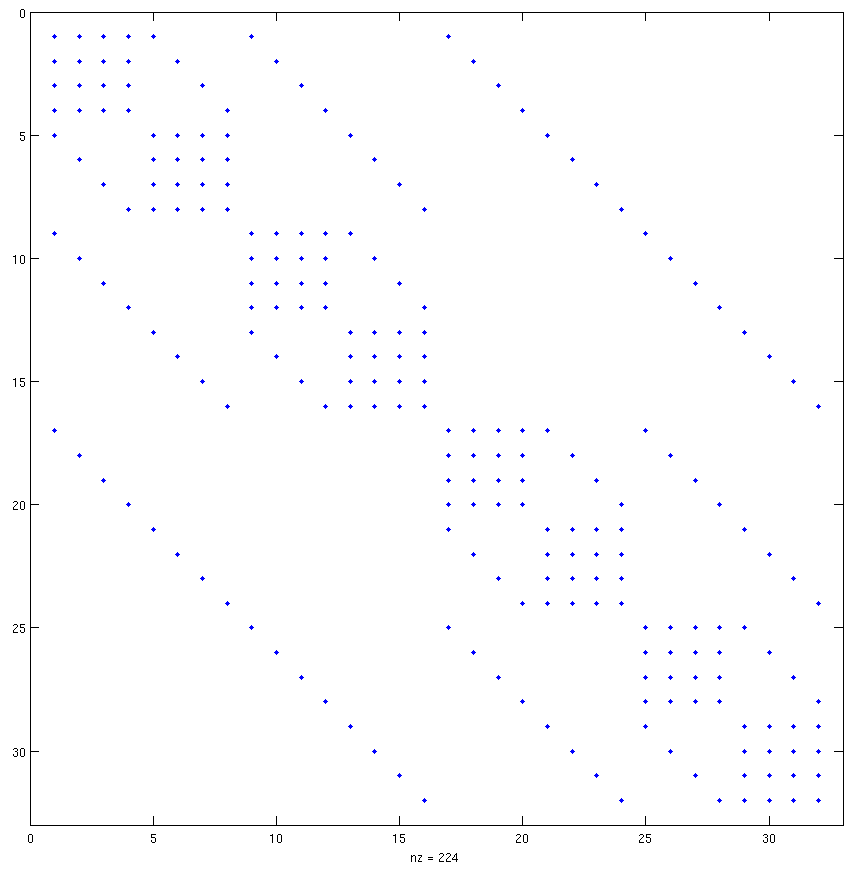
\includegraphics[width=3in]{chapters/spn_equations/group1.png}
  \end{center}
  \caption{\textbf{Sparsity pattern for 1-group $SP_7$
      discretization.} \textit{A $2\times 2 \times 2$ element mesh was
      used to show detail of the blocks formed by the discretization.}}
  \label{fig:group1}
\end{figure}
\begin{figure}[t!]
  \begin{center}
    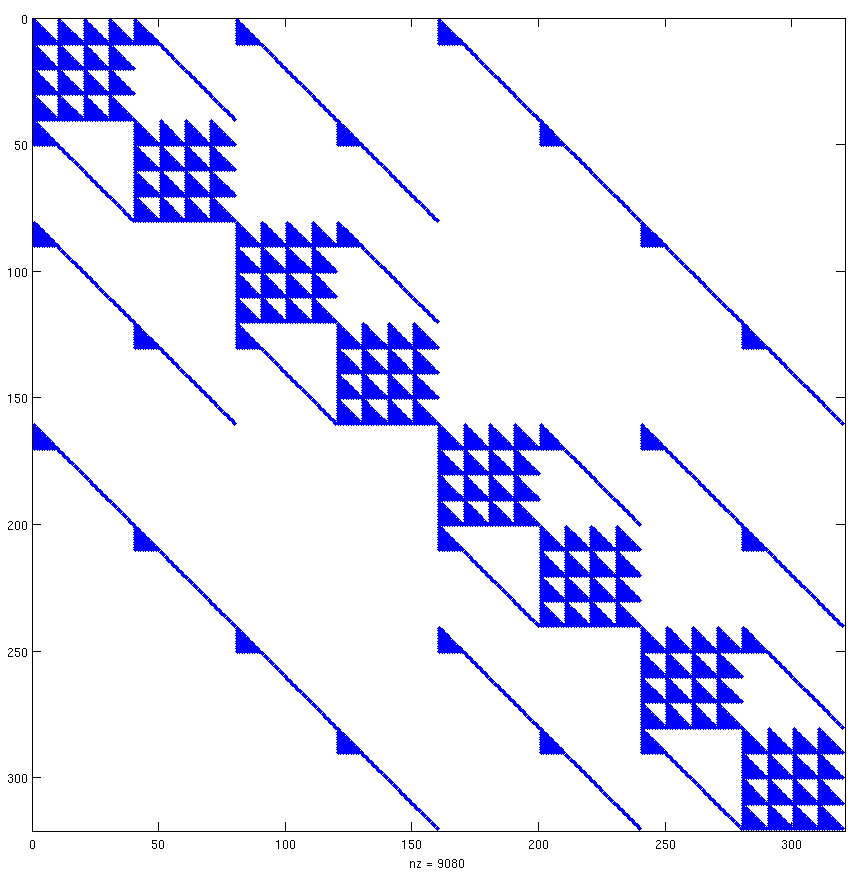
\includegraphics[width=3in]{chapters/spn_equations/group10ds.png}
  \end{center}
  \caption{\textbf{Sparsity pattern for 10-group $SP_7$ discretization
      with downscatter only.} \textit{A $2\times 2 \times 2$ element
      mesh was used to show detail of the blocks formed by the
      discretization.}}
  \label{fig:group10ds}
\end{figure}
\begin{figure}[t!]
  \begin{center}
    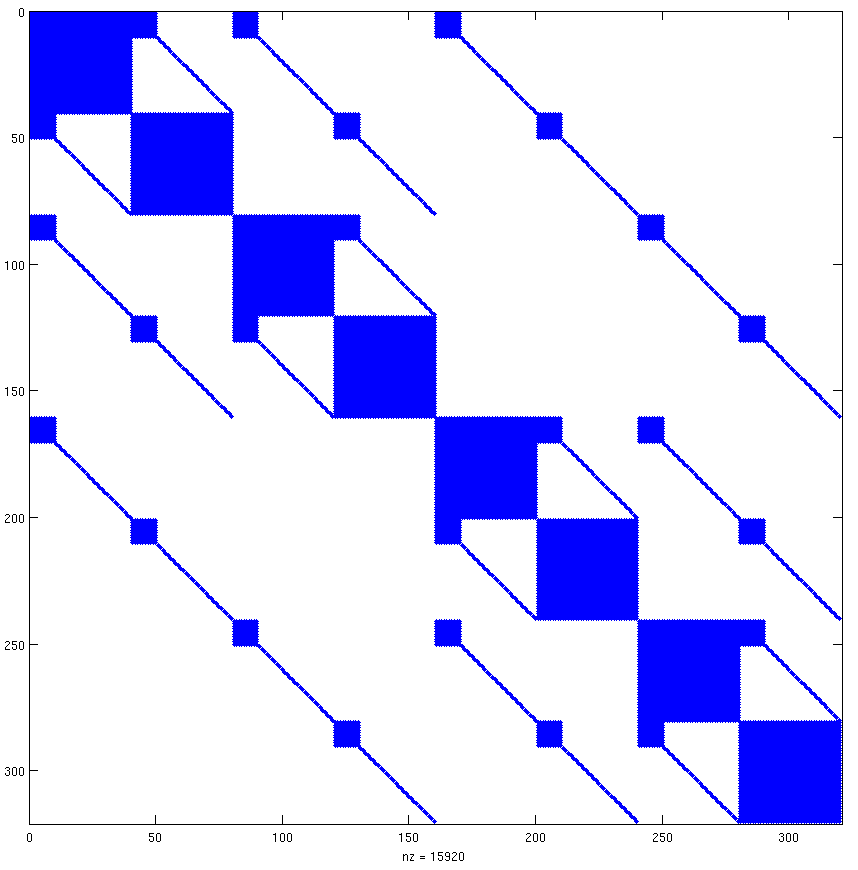
\includegraphics[width=3in]{chapters/spn_equations/group10us.png}
  \end{center}
  \caption{\textbf{Sparsity pattern for 10-group $SP_7$ discretization
      with downscatter and upscatter.} \textit{A $2\times 2 \times 2$ element
      mesh was used to show detail of the blocks formed by the
      discretization.}}
  \label{fig:group10us}
\end{figure}
We note a few key features of the sparsity plots. The first is that
for multigroup problems without full upscatter and downscatter
(i.e. Figure~\ref{fig:group10ds}), the resulting matrix is asymmetric
and therefore a linear solver that can handle asymmetric linear
systems is required. Nearly all problems of interest will not have
full upscattering or downscattering. Second we note the largely
diagonal character of these systems, although the blocks from
Eq~(\ref{eq:A_block_matrix}) are readily apparent. Our first attempt
at preconditioning this system will be to use the point Jacobi
preconditioning from \S\ref{subsubsec:basic_mcsa_preconditioning} due
to this diagonal form.

\subsection{Point Jacobi Spectral Analysis Results}
\label{subsec:spn_analysis_results}
Spectral radius computations were performed for the cases described
above for the point Jacobi preconditioned iteration matrix $\ve{H} =
\ve{I}-\ve{M}^{-1}\ve{A}$ with $\ve{M} =
diag(\ve{A})$. Table~\ref{tab:group1pj} gives the results for the
1-group case, Table~\ref{tab:group10dspj} for the 10-group case with
full downscatter only and Table~\ref{tab:group10uspj} for the 10-group
case with full downscatter and full upscatter.
\begin{table}[h!]
  \begin{center}
    \begin{tabular}{cccccc}\hline\hline
      \multicolumn{1}{c}{}& 
      \multicolumn{1}{c}{}& 
      \multicolumn{1}{c}{}& 
      \multicolumn{1}{c}{$SP_N$ Order}& 
      \multicolumn{1}{c}{}& 
      \multicolumn{1}{c}{} \\
       &   & \textbf{1} & \textbf{3} & \textbf{5} & \textbf{7}  \\
       & \textbf{0} & 0.0635 & 0.6722 & 1.3144 & 1.976 \\
       & \textbf{1} & 0.0666 & 0.6728 & 1.3141 & 1.9755 \\
      $P_N$ Order & \textbf{3} & 0.0666 & 0.6822 & 1.3141 & 1.9755 \\
       & \textbf{5} & 0.0666 & 0.6822 & 1.3278 & 1.9847 \\
       & \textbf{7} & 0.0666 & 0.6822 & 1.3278 & 1.9917 \\
      %%
      \hline\hline
    \end{tabular}
  \end{center}
  \caption{\textbf{Spectral radius results for the point Jacobi
      preconditioned iteration matrix with 1 energy group.}}
  \label{tab:group1pj}
\end{table}
\begin{table}[h!]
  \begin{center}
    \begin{tabular}{cccccc}\hline\hline
      \multicolumn{1}{c}{}& 
      \multicolumn{1}{c}{}& 
      \multicolumn{1}{c}{}& 
      \multicolumn{1}{c}{$SP_N$ Order}& 
      \multicolumn{1}{c}{}& 
      \multicolumn{1}{c}{} \\
       &   & \textbf{1} & \textbf{3} & \textbf{5} & \textbf{7}  \\
       & \textbf{0} & 0.0655 & 0.677 & 1.32 & 1.982 \\
       & \textbf{1} & 0.071 & 0.6777 & 1.319 & 1.982 \\
      $P_N$ Order & \textbf{3} & 0.071 & 0.687 & 1.327 & 1.9872 \\
       & \textbf{5} & 0.071 & 0.687 & 1.336 & 1.997 \\
       & \textbf{7} & 0.071 & 0.687 & 1.336 & 1.9995 \\
      %%
      \hline\hline
    \end{tabular}
  \end{center}
  \caption{\textbf{Spectral radius results for the point Jacobi
      preconditioned iteration matrix with 10 energy groups and full
      downscatter.}}
  \label{tab:group10dspj}
\end{table}
\begin{table}[h!]
  \begin{center}
    \begin{tabular}{cccccc}\hline\hline
      \multicolumn{1}{c}{}& 
      \multicolumn{1}{c}{}& 
      \multicolumn{1}{c}{}& 
      \multicolumn{1}{c}{$SP_N$ Order}& 
      \multicolumn{1}{c}{}& 
      \multicolumn{1}{c}{} \\
       &   & \textbf{1} & \textbf{3} & \textbf{5} & \textbf{7}  \\
       & \textbf{0} & 0.7283 & 0.81 & 1.47 & 2.1446 \\
       & \textbf{1} & 0.7317 & 0.8 & 1.46 & 2.1368 \\
      $P_N$ Order & \textbf{3} & 0.7317 & 0.91 & 1.526 & 2.2274 \\
       & \textbf{5} & 0.7317 & 0.91 & 1.5344 & 2.2562 \\
       & \textbf{7} & 0.7317 & 0.91 & 1.5345 & 2.2842 \\
      %%
      \hline\hline
    \end{tabular}
  \end{center}
  \caption{\textbf{Spectral radius results for the point Jacobi
      preconditioned iteration matrix with 10 energy groups, full
      downscatter and full upscatter.}}
  \label{tab:group10uspj}
\end{table}
It is readily apparent from the tabulated data that point Jacobi
preconditioning is insufficient. For problems of order $SP_5$ and
$SP_7$, the method will not converge at all and for the upscatter case
with $SP_3$ the spectral radius is still quite large for large $P_N$
orders and therefore convergence is expected to be slow. These
eigenvalues signal a need for a better preconditioning strategy to
both ensure and improve convergence for Monte Carlo methods.

\subsection{Block Jacobi Preconditioning}
\label{sec:spn_preconditioning}
If Monte Carlo methods are to be used to solve the $SP_N$ system of
equations, a different preconditioning strategy is required in order
to ensure convergence for systems of all $SP_N$ and $P_N$ orders with
arbitrary energy group structures. As another means of achieving this,
we look back to the sparsity plots we generated in
Figures~\ref{fig:group1}, \ref{fig:group10ds} and \ref{fig:group10us}
as well as the multigroup $SP_N$ equations. Initially, the diagonal
character of the system led us to try point Jacobi preconditioning
with only marginal results. From the sparsity plots we note the block
structure that ultimately arises from the multigroup scattering
matrices and their insertion into Eq~(\ref{eq:A_block_matrix}). When
full upscatter and downscatter are used the resulting blocks are
completely dense while only downscatter gives a lower triangular
scattering matrix and the block structure shown in
Figure~\ref{fig:group10ds}.

Based on this both block and diagonally dominant structure for
matrices formed by the general multigroup $SP_N$ equations, we instead
choose \textit{block Jacobi} preconditioning as a left preconditioner
for the system. Like point Jacobi preconditioning, block Jacobi
preconditioning extracts the diagonal elements of the matrix as the
preconditioner where now the elements extracted are the blocks on the
diagonal as shown on the left side of
Figure~\ref{fig:block_jacobi_ex}. Shown on the right side of
Figure~\ref{fig:block_jacobi_ex}, inversion of the preconditioner is
trivial with each diagonal block inverted separately. For the $SP_N$
equations, Eq~(\ref{eq:A_block_matrix}) gives a block size of
$N_g\times(N+1)/2$.
\begin{figure}[t!]
  \begin{center}
    \scalebox{1.5}{
    \input{chapters/spn_equations/block_jacobi.pdftex_t} }
  \end{center}
  \caption{\textbf{Block Jacobi preconditioning strategy used for the
      $SP_N$ equations.} \textit{Left: The preconditioner is formed by
      the diagonal blocks of the matrix. Right: Inversion of the
      preconditioner is trivial and decoupled by block.}}
  \label{fig:block_jacobi_ex}
\end{figure}
The inversion of this preconditioner is trivial as shown on the right
side of Figure~\ref{fig:block_jacobi_ex}. Each block can be inverted
individually and combined to form the inverse. In addition, in the
limit of a block size of one, the block Jacobi method reduces to the
point Jacobi method. For high performance implementations this has
several attractive properties. First, the blocks in the matrix come
from the energy/angle discretization of the transport equation as
given by Eq~(\ref{eq:A_block_matrix}). Each block on the diagonal is
bound to a mesh element in the system (note there are 8 blocks on the
diagonal in each of the sparsity patterns with a mesh of $2 \times 2
\times 2$) and therefore we expect the matrix elements forming the
block to be entirely local. Second, these blocks are typically dense
and nearly lower triangular for many transport problems meaning that
established dense matrix methods can be used for fast inversion.

\subsection{Block Jacobi Spectral Analysis Results}
\label{subsec:spn_analysis_results}
Spectral radius computations for the block Jacobi preconditioned
iteration matrix were performed for the same problems as the point
Jacobi preconditioned case. Table~\ref{tab:group1bj} gives the results
for the 1-group case, Table~\ref{tab:group10dsbj} for the 10-group
case with full downscatter only and Table~\ref{tab:group10usbj} for
the 10-group case with full downscatter and full upscatter. A block
size of $N_g\times(N+1)/2$ was used for the preconditioner in all
cases.
\begin{table}[h!]
  \begin{center}
    \begin{tabular}{cccccc}\hline\hline
      \multicolumn{1}{c}{}& 
      \multicolumn{1}{c}{}& 
      \multicolumn{1}{c}{}& 
      \multicolumn{1}{c}{$SP_N$ Order}& 
      \multicolumn{1}{c}{}& 
      \multicolumn{1}{c}{} \\
       &   & \textbf{1} & \textbf{3} & \textbf{5} & \textbf{7}  \\
       & \textbf{0} & 0.0635 & 0.1269 & 0.1444 & 0.1513 \\
       & \textbf{1} & 0.0666 & 0.1315 & 0.1474 & 0.1534 \\
      $P_N$ Order & \textbf{3} & 0.0666 & 0.1365 & 0.154 & 0.1592 \\
       & \textbf{5} & 0.0666 & 0.1365 & 0.1562 & 0.163 \\
       & \textbf{7} & 0.0666 & 0.1365 & 0.1562 & 0.164 \\
      %%
      \hline\hline
    \end{tabular}
  \end{center}
  \caption{\textbf{Spectral radius results for the block Jacobi
      preconditioned iteration matrix with 1 energy group.}}
  \label{tab:group1bj}
\end{table}
\begin{table}[h!]
  \begin{center}
    \begin{tabular}{cccccc}\hline\hline
      \multicolumn{1}{c}{}& 
      \multicolumn{1}{c}{}& 
      \multicolumn{1}{c}{}& 
      \multicolumn{1}{c}{$SP_N$ Order}& 
      \multicolumn{1}{c}{}& 
      \multicolumn{1}{c}{} \\
       &   & \textbf{1} & \textbf{3} & \textbf{5} & \textbf{7}  \\
       & \textbf{0} & 0.0647 & 0.1275 & 0.1449 & 0.1514 \\
       & \textbf{1} & 0.0686 & 0.1338 & 0.1484 & 0.1547 \\
      $P_N$ Order & \textbf{3} & 0.0687 & 0.1399 & 0.1582 & 0.1625 \\
       & \textbf{5} & 0.0692 & 0.1399 & 0.1582 & 0.1657 \\
       & \textbf{7} & 0.0678 & 0.1393 & 0.1624 & 0.166 \\
      %%
      \hline\hline
    \end{tabular}
  \end{center}
  \caption{\textbf{Spectral radius results for the block Jacobi
      preconditioned iteration matrix with 10 energy groups and full
      downscatter.}}
  \label{tab:group10dsbj}
\end{table}
\begin{table}[h!]
  \begin{center}
    \begin{tabular}{cccccc}\hline\hline
      \multicolumn{1}{c}{}& 
      \multicolumn{1}{c}{}& 
      \multicolumn{1}{c}{}& 
      \multicolumn{1}{c}{$SP_N$ Order}& 
      \multicolumn{1}{c}{}& 
      \multicolumn{1}{c}{} \\
       &   & \textbf{1} & \textbf{3} & \textbf{5} & \textbf{7}  \\
       & \textbf{0} & 0.1887 & 0.2267 & 0.2285 & 0.2286 \\
       & \textbf{1} & 0.4535 & 0.5044 & 0.5045 & 0.5045 \\
      $P_N$ Order & \textbf{3} & 0.4535 & 0.6453 & 0.6506 & 0.6506 \\
       & \textbf{5} & 0.4535 & 0.6453 & 0.6802 & 0.6818 \\
       & \textbf{7} & 0.4535 & 0.6453 & 0.6802 & 0.6927 \\
      %%
      \hline\hline
    \end{tabular}
  \end{center}
  \caption{\textbf{Spectral radius results for the block Jacobi
      preconditioned iteration matrix with 10 energy groups, full
      downscatter and full upscatter.}}
  \label{tab:group10usbj}
\end{table}

From the tabulated block Jacobi data it is clear that this is a viable
preconditioning choice for all $SP_N$ problems in term of Monte Carlo
solution methods. All cases were observed to have a spectral radius
below unity and often significantly smaller than that, greatly
improving convergence rates over the point Jacobi preconditioned
problem. Based on these results, the block Jacobi method should be the
first preconditioning strategy applied to more complicated problems
representative of physical systems.
\clearpage

%%---------------------------------------------------------------------------%%
\section{Fuel Assembly Criticality Calculations}
\label{sec:fuel_assembly_calcs}
Fuel assembly calculations are a critical piece of nuclear engineering
infrastructure for reactor core analysis and design. At this level,
individual fuel pins may be resolved at fine resolution in a variety
of configurations. As a sophisticated problem of interest to push the
limits of MCSA, a hot zero-power $17 \times 17$ pin assembly will be
used with varying energy group structure and $SP_N$ discretization in
a criticality calculation. A cross section along the vertical axis
showing homogenized fuel pin materials and the associated grid is
given by Figure~\ref{fig:problem3_radial_mat} while a cross section of
the materials configuration along the horizontal axis is given by
Figure~\ref{fig:problem3_axial_mat}. A detailed view of the assembly
bottom is given in Figure~\ref{fig:problem3_end}. On the top and
bottom of the assembly, vacuum conditions are used as well as on the
top and right boundaries in
Figure~\ref{fig:problem3_radial_mat}. Reflecting conditions are used
on the left and bottom boundaries of
Figure~\ref{fig:problem3_radial_mat}, effectively giving a
representation of one quarter of the assembly.
\begin{figure}[t!]
  \begin{center}
    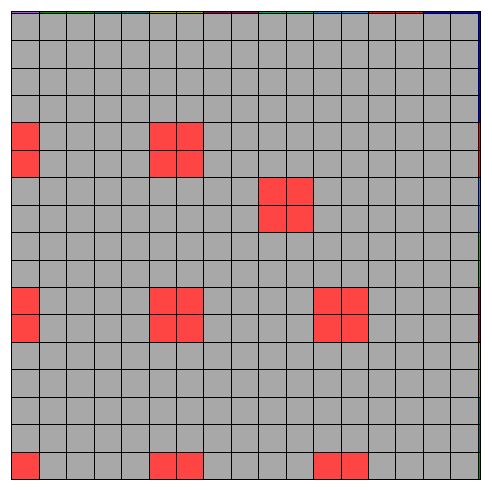
\includegraphics[width=4in]{chapters/spn_equations/problem3_radial_mat.png}
  \end{center}
  \caption{\textbf{Fuel assembly mesh and geometry cross section.}
    \textit{Reflecting boundaries are used on the left and lower
      boundaries to create a complete $17 \times 17$ assembly
      geometry. Gray regions are homogenized fuel and red regions are
      homogenzied moderator. Each fuel pin is resolved by a $2 \times
      2$ mesh.}}
  \label{fig:problem3_radial_mat}
\end{figure}
\begin{figure}[t!]
  \begin{center}
    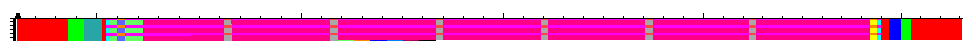
\includegraphics[width=6.0in]{chapters/spn_equations/problem3_axial_mat.png}
  \end{center}
  \caption{\textbf{Fuel assembly geometry cross section.}  \textit{The
      geometry is subdivided along the axial direction into 50 zones
      spaced to capture material boundaries. Important details include
      spacer grids along the length of the fuel pins and reactor core
      structures on the top and bottom of the assembly. Lighter purple
      material in the center of the assembly is moderator and darker
      purple material fuel.}}
  \label{fig:problem3_axial_mat}
\end{figure}
\begin{figure}[t!]
  \begin{center}
    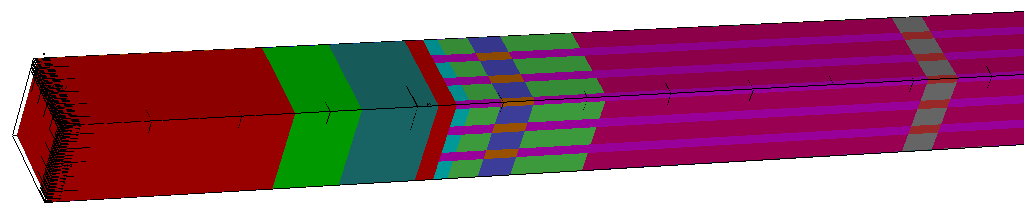
\includegraphics[width=6.0in]{chapters/spn_equations/problem3_end.png}
  \end{center}
  \caption{\textbf{Fuel assembly geometry end detail.}
    \textit{Reactor core structure including spacer grids and plenum
      has been included. Lighter purple material on the right of the
      figure is moderator and darker purple material fuel.}}
  \label{fig:problem3_end}
\end{figure}
Significant geometric details are contained in the model including
spacer grids, fuel pins with homogenized cladding and gas gap, core
plenum, and moderator with boron. Group cross sections and other
discrete nuclear data are generated as needed by a cross-section
processing module dependent on the meshing parameters used to
discretize the geometry and single-dimension pin-cell calculations for
intial flux spectrum generation. Table~\ref{tab:problem3_parameters}
gives the primary design parameters for the fuel assembly
calculations.
\begin{table}[h!]
  \begin{center}
    \begin{tabular}{ll}\hline\hline
      \multicolumn{1}{l}{\textbf{Parameter}} & 
      \multicolumn{1}{l}{\textbf{Value}} \\
      Power Level & 0 MW \\
      Inlet Temperature & 326.85C \\
      Fuel Temperature & 600C \\
      Boron Concentration & 1300 ppm \\
      Moderator Density & 0.743 g/cc \\
      Helium Density & \sn{1.79}{-4} g/cc \\
      Zirconium Density & 6.56 g/cc \\
      Stainless Steel Density & 8.0 g/cc \\
      Inconel Density & 8.19 g/cc \\
      UO2 Density & 10.257 g/cc \\
      Fuel Pin Radius (w/o clad) & 0.4096 cm \\
      %%
      \hline\hline
    \end{tabular}
  \end{center}
  \caption{\textbf{Design parameters for the $17 \times 17$ pin fuel
      assembly criticality calculation.}}
  \label{tab:problem3_parameters}
\end{table}

To generate the multiplication factor and steady-state flux
distribution for this problem, at every eigenvalue iteration MCSA is
used to solve the resulting $SP_N$ problem using the provided fission
source. Algorithm~\ref{alg:power_iteration} presents the use of MCSA
within a power iteration strategy to find the multiplication factor.
\begin{algorithm}[h!]
  \caption{Power Iteration MCSA Scheme}
  \label{alg:power_iteration}
  \begin{algorithmic}
    \State $k_0 =$ initial guess
    \State $\mathbf{\Phi}_0 =$ initial guess
    \State $n = 0$
    \While{$|\frac{k^n - k^{n-1}}{k^n}| < \epsilon$}
    \Comment{Iterate until convergence of the eigenvalue}
    \State $\mathbf{M} \mathbf{\Phi}^{n+1} = \frac{1}{k^n} \mathbf{F} \mathbf{\Phi}^n$
    \Comment{Solve for the new flux state with MCSA}
    \State $k^{n+1} = k^n \frac{\int \mathbf{F} \mathbf{\Phi}^{n+1} d\mathbf{r}}{\int
      \mathbf{F} \mathbf{\Phi}^n d\mathbf{r}}$
    \Comment{Update the multiplication factor}
    \State $n = n+1$
    \EndWhile
  \end{algorithmic}
\end{algorithm}
Here, $\mathbf{M}$ is the transport operator generated on the
left-hand side of the $SP_N$ discretization, $\mathbf{F}$ is the
fission matrix, and $\mathbf{\Phi}$ the multigroup neutron flux. This
problem is significantly more complicated than the simple test problem
used for the previous spectral analysis. Fission has been introduced
into the set of equations and the addition of moderator into the
system will increase the amount of scattering, creating a
significantly more difficult problem manifesting itself in an
iteration matrix with a larger spectral radius. When using MCSA, the
linear operator applied to $\mathbf{\Phi}^{n+1}$ at each eigenvalue
iteration will dictate convergence and remain unchanged throughout the
computation\footnote{The operator will change if, for example, physics
  feedback through temperature or potentially burnup is
  considered. These additional physics will modify the cross sections
  used to assemble $\mathbf{M}$. The calculations presented here will
  consist of a single eigenvalue calculation with a static
  $\mathbf{M}$.} while the addition of fission to the system will only
modify the source of neutrons and the multiplication factor while not
affecting Monte Carlo transport.

\subsection{Preliminary Jacobi Preconditioned Calculations}
\label{subsec:jacobi_prec_assembly_calc}
Based on the success of block Jacobi preconditioning with the test
problem used for the spectral radius parameter study, we use it first
to solve the $17 \times 17$ fuel assembly problem. A single energy
group problem was first solved with $SP_1$ discretization, effectively
giving the one-speed neutron diffusion system for the fuel assembly
resulting in 20,088 degrees of freedom in the
problem. Figure~\ref{fig:block_jacobi_res_mcsa} gives the residual
infinity norm as a function of iteration for the MCSA linear solve in
the first eigenvalue iteration using 25,000 stochastic histories at
every iteration for the adjoint Neumann-Ulam solve.
\begin{figure}[t!]
  \begin{center}
    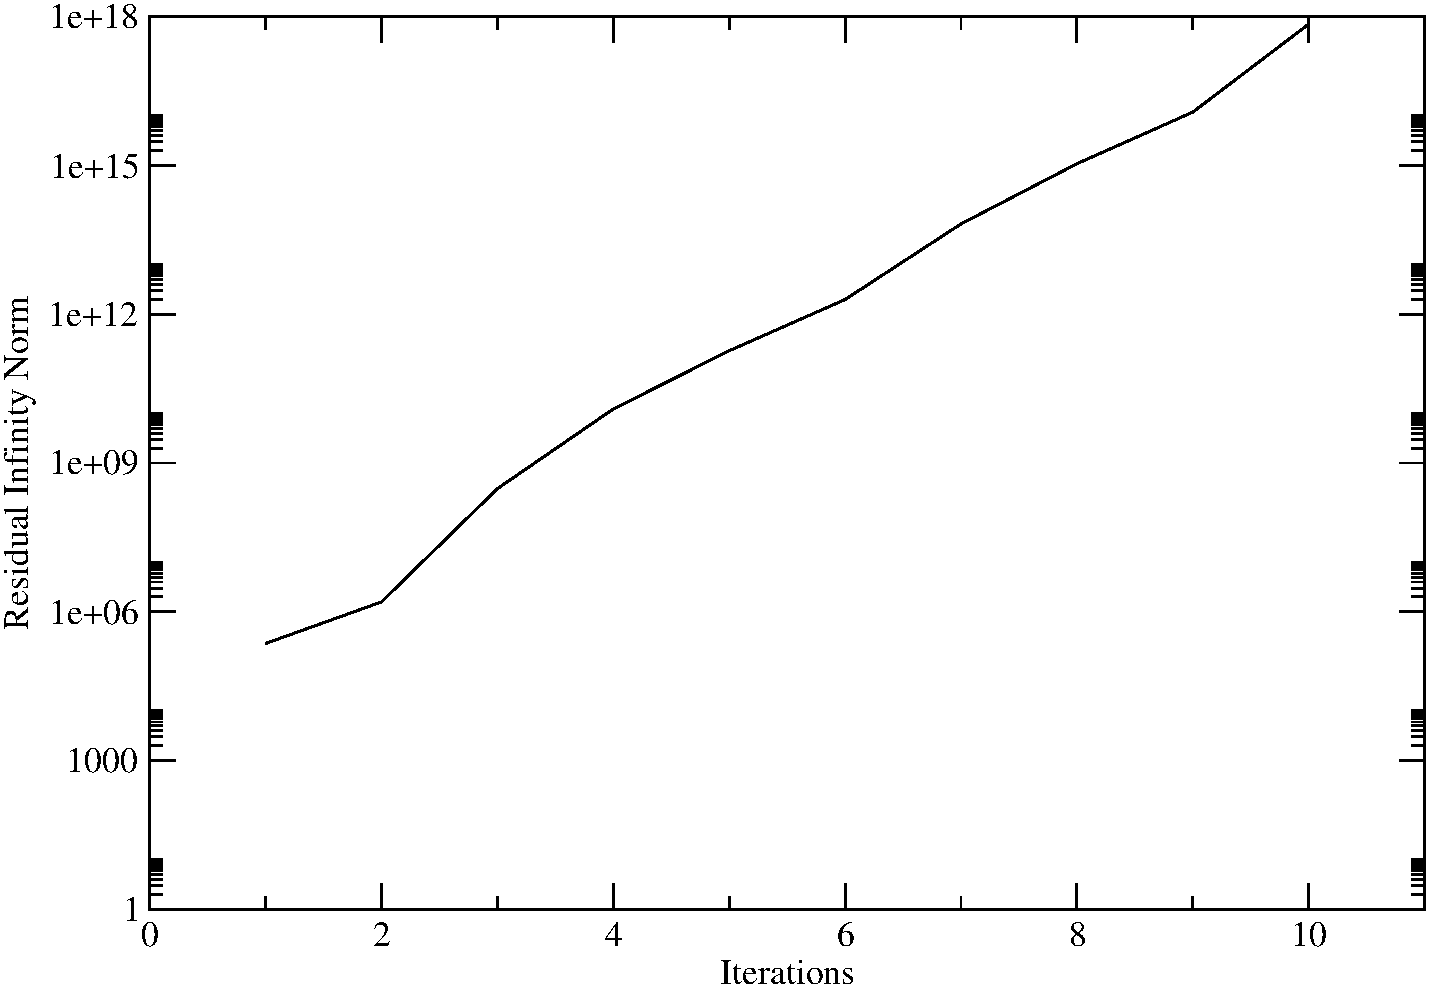
\includegraphics[width=5in]{chapters/spn_equations/block_jacobi_res.pdf}
  \end{center}
  \caption{\textbf{Residual infinity norm vs. iteration for the block
      Jacobi preconditioned MCSA solve during the first eigenvalue
      iteration of the 1-group $17 \times 17$ fuel assembly problem.}
    \textit{Convergence was not achieved with the block Jacobi
      preconditioned method.}}
  \label{fig:block_jacobi_res_mcsa}
\end{figure}
Convergence was not achieved as noted by the rapid rise in the
residual over a few iterations. Based on the spectral radius
computations performed, these results are not in line with
expectations for this problem. Additional computations performed with
\sn{1}{6} histories per iteration exhibited the same divergent
behavior at a significant computational cost and compute time. Even if
the problem may be ill-conditioned, we do expect convergence of
MCSA. To investigate further, a block Jacobi preconditioned Richardson
iteration was used to solve the same
problem. Figure~\ref{fig:block_jacobi_res_richardson} gives the
residual infinity norm as a function of iteration for the Richardson
linear solve in the first eigenvalue iteration.
\begin{figure}[t!]
  \begin{center}
    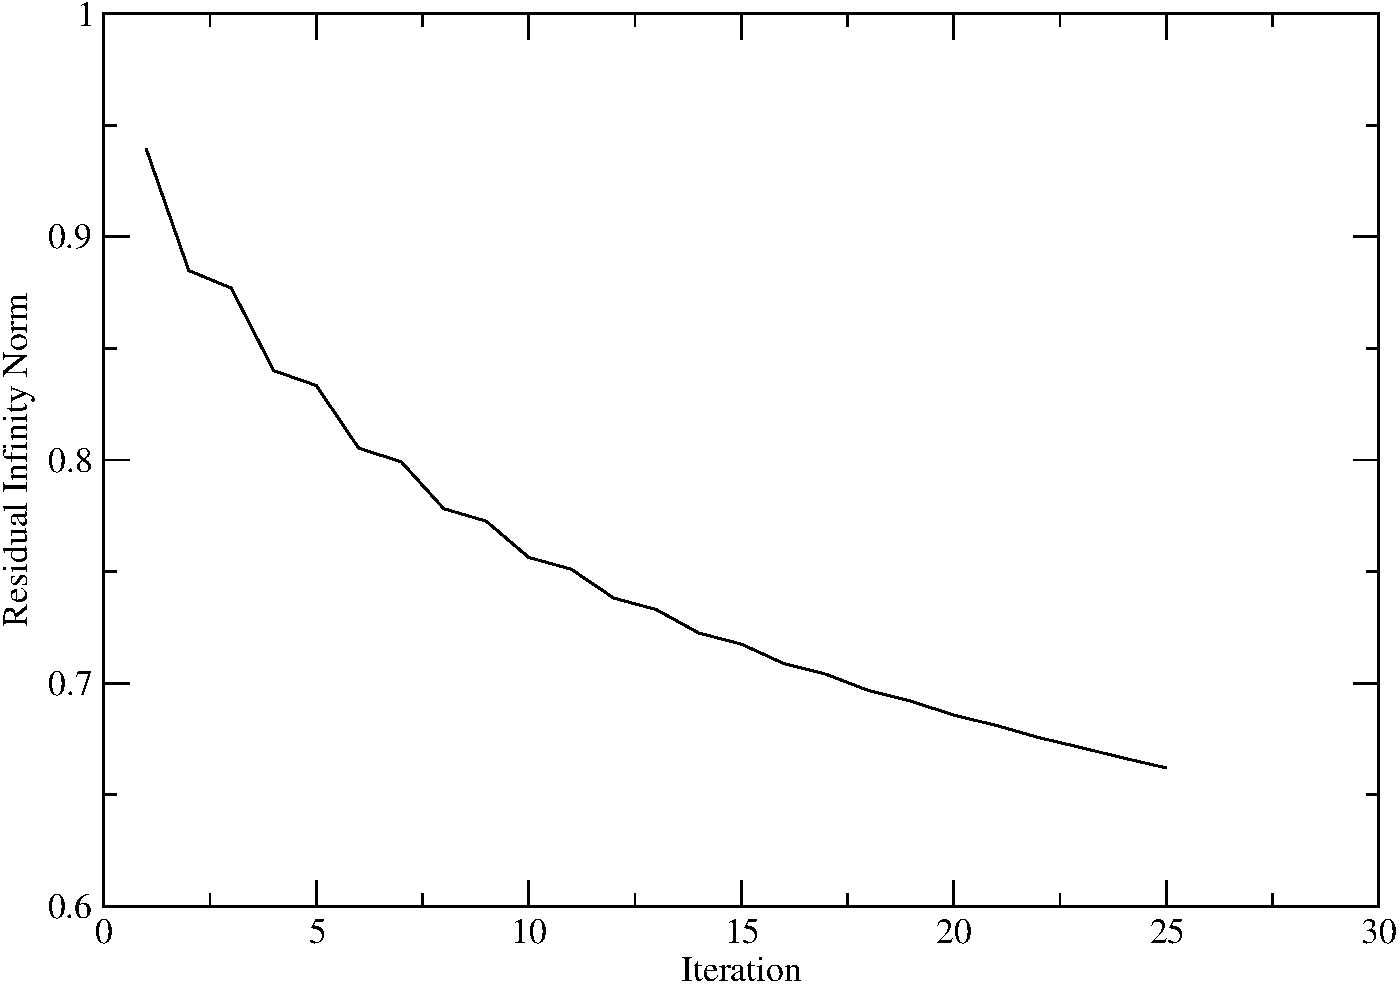
\includegraphics[width=5in]{chapters/spn_equations/block_jacobi_rich_res.pdf}
  \end{center}
  \caption{\textbf{Residual infinity norm vs. iteration for the block
      Jacobi preconditioned Richardson solve during the first
      eigenvalue iteration of the 1-group $17 \times 17$ fuel assembly
      problem.}  \textit{A spectral radius near 1 was observed for the
      iteration matrix.}}
  \label{fig:block_jacobi_res_richardson}
\end{figure}
Poor converge is observed for the Richardson iteration, however,
convergence is achieved meaning that the preliminary criteria needed
to satisfy MCSA convergence has also been met. The number of
iterations required for the Richardson iteration to converge will give
an approximation for the spectral radius via
Eq~(\ref{eq:linear_k_iter_norm3}). With 7291 iterations required to
converge to a tolerance of $\sn{1}{-6}$, $\rho(\mathbf{H}) \approx
0.998$, nearing the limits of MCSA applicability and well beyond the
spectral radii generated in the initial spectral analysis.

Based on these results, it then appears that even if the simple
criteria of a spectral radius of less than one is met and the
Richardson iteration will converge with the same preconditioning, MCSA
still may not converge. We then expect the issue to reside with the
Neumann-Ulam solve providing the correction as the Richardson
iteration is known to provide the correct result. Furthermore, the
fact that the spectral radius is less than one means that the
stochastic histories in the block Jacobi preconditioned Neumann-Ulam
method are eventually being terminated by the weight cutoff as no
artificial absorption was used for these preliminary
calculations. Based on this, the correction being generated by the
Neumann-Ulam solve is the component of MCSA causing a divergent
solution.

\subsection{MCSA Breakdown}
\label{subsec:mcsa_break_down}
For the fuel assembly problem, the initial block Jacobi
preconditioned\footnote{For 1-group $SP_1$ problems, the block size is
  1, giving a point Jacobi preconditioner.}  calculations used a
one-speed $SP_1$ discretization, effectively giving a diffusion
system. To study the breakdown of MCSA at iteration matrix spectral
radii near one, we will use a simpler homogoneous 2-dimensional
one-speed neutron diffusion system to isolate this behavior. In this
system, we can vary the cross sections while maintaining a fixed grid
in order to achieve varying spectral radii. For these studies, we
neglect fission as MCSA behavior is dictated by the transport operator
$\mathbf{M}$ in an eigenvalue scheme with the fission matrix used to
generate a fixed source.

\subsubsection{Model Diffusion Problem}
\label{subsec:model_problem}
For our breakdown study, we choose the one-speed, two-dimensional
neutron diffusion equation as a model problem
\citep{duderstadt_nuclear_1976}:
\begin{equation}
  -\boldsymbol{\nabla} \cdot D \boldsymbol{\nabla} \phi + \Sigma_a
  \phi = S\:,
  \label{eq:diffusion_eq}
\end{equation}
where $\phi$ is the neutron flux, $\Sigma_a$ is the absorption cross
subsection, and $S$ is the source of neutrons. In addition, $D$ is the
diffusion coefficient defined as:
\begin{equation}
  D = \frac{1}{3 ( \Sigma_t - \bar{\mu}\Sigma_s )}\:,
  \label{eq:diffusion_coeff}
\end{equation}
where $\Sigma_s$ is the scattering cross subsection, $\Sigma_t = \Sigma_a
+ \Sigma_s$ is the total cross subsection, and $\bar{\mu}$ is the cosine
of the average scattering angle. For simplicity, we will take
$\bar{\mu} = 0$ for our analysis giving $D=(3 \Sigma_t)^{-1}$. In
addition, to further simplify we will assume a homogeneous domain such
that the cross subsections remain constant throughout. Doing this permits
us to rewrite Eq~(\ref{eq:diffusion_eq}) as:
\begin{equation}
  -D \boldsymbol{\nabla}^2 \phi + \Sigma_a \phi = S\:.
  \label{eq:diffusion_eq_simple}
\end{equation}

We choose a finite difference scheme on a square Cartesian grid to
discretize the problem. For the Laplacian, we choose the 9-point
stencil shown in Figure~\ref{fig:stencil} over a grid of size $h$
\citep{leveque_finite_2007}:
\begin{multline}
  \nabla^2_9\phi = \frac{1}{6h^2}[4 \phi_{i-1,j} + 4 \phi_{i+1,j}
    + 4 \phi_{i,j-1} + 4 \phi_{i,j+1} + \phi_{i-1,j-1}\\ +
    \phi_{i-1,j+1} + \phi_{i+1,j-1} + \phi_{i+1,j+1} - 20
    \phi_{i,j}]\:.
  \label{eq:nine_point_stencil}
\end{multline}
\begin{figure}[t!]
  \begin{center}
    \scalebox{1.25}{\input{chapters/spn_equations/stencil.pdftex_t}}
  \end{center}
  \caption{\textbf{Nine-point Laplacian stencil.}}
  \label{fig:stencil}
\end{figure}
We then have the following linear system to solve:
\begin{multline}
  -\frac{1}{6h^2}[4 \phi_{i-1,j} + 4 \phi_{i+1,j} + 4
    \phi_{i,j-1} + 4 \phi_{i,j+1} + \phi_{i-1,j-1}\\ + \phi_{i-1,j+1}
    + \phi_{i+1,j-1} + \phi_{i+1,j+1} - 20 \phi_{i,j}] + \Sigma_a
  \phi_{i,j} = s_{i,j}\:,
  \label{eq:fd_system}
\end{multline}
and in operator form:
\begin{equation}
  \ve{D}\boldsymbol{\phi}=\ve{s}\:,
  \label{eq:operator_system}
\end{equation}
where $\ve{D}$ is the diffusion operator, $\ve{s}$ is the source in
vector form and $\boldsymbol{\phi}$ is the vector of unknown fluxes.

To close the system, a set of boundary conditions is required. In the
case of a non-reentrant current condition applied to all global
boundaries of the domain, we choose the formulation of Duderstadt by
assuming the flux is zero at some ghost point beyond the
grid. Consider for example the equations on the $i=0$ boundary of the
domain:
\begin{multline}
  -\frac{1}{6h^2}[4 \phi_{-1,j} + 4 \phi_{1,j} + 4 \phi_{0,j-1} +
    4 \phi_{0,j+1} + \phi_{-1,j-1}\\ + \phi_{-1,j+1} + \phi_{1,j-1} +
    \phi_{1,j+1} - 20 \phi_{0,j}] + \Sigma_a \phi_{0,j} = s_{0,j}\:.
  \label{eq:x_min_bnd}
\end{multline}
Here we note some terms where $i=-1$ and therefore are representative
of grid points beyond the boundary of the domain. We set the flux at
these points to be zero, giving a valid set of equations for the $i=0$
boundary:
\begin{multline}
  -\frac{1}{6h^2}[4 \phi_{1,j} + 4 \phi_{0,j-1} + 4 \phi_{0,j+1}
    \\ + \phi_{-1,j+1} + \phi_{1,j-1} + \phi_{1,j+1} - 20 \phi_{0,j}]
  + \Sigma_a \phi_{0,j} = s_{0,j}\:.
  \label{eq:x_min_bnd_2}
\end{multline}
We repeat this procedure for the other boundaries of the domain. For
reflecting boundary conditions, the net current across a boundary is
zero.

\subsubsection{MCSA Breakdown Analysis}
\label{subsubsec:breakdown_analysis}
For each solver and estimator combination, the spectral radius of the
iteration matrix was varied by changing the absorption cross section
while fixing the grid size and scattering cross section. At each
solve, a minimum of one stochastic history per degree of freedom (DOF)
in the problem was used to compute the Monte Carlo correction. If the
solver could not converge in less than 100 iterations, the number of
histories was increased by increments of 5,000 until convergence was
achieved in less than 100 iterations. The number of iterations
required to converge MCSA and the time to converge was recorded as a
means to capture the breakdown. 

Figure~\ref{fig:breakdown_iterations} gives the number of iterations
required to converge for the chosen number of histories per iteration
given by Figure~\ref{fig:breakdown_histories} using the adjoint solver
with the collision and expected value estimators and the forward
solver with the collision estimator. For spectral radii less than
0.97, all MCSA problems converged with 1 history per DOF (10,000 for
this problem) with the number of iterations required to converge
increasing. Near a spectral radius of 0.97, the number of histories
required to converge MCSA in less than 100 iterations takes a dramatic
rise that exhibits neither exponential nor power law behavior. As the
spectral radius approaches 1, the number of histories required becomes
significant and effectively intractable. Even with this simple
diffusion problem, the behavior is consistent with that oberseved for
the fuel assembly problem with $SP_1$ discretization. In that case, we
estimated a spectral radius of $\approx 0.998$, larger than any of the
spectral radii that could be computed within even 90 minutes of
compute time for this simple two dimensional problem. For that
problem, even 1,000,000 histories ($\approx 50$ per DOF) was not
enough to provide convergence.
\begin{figure}[t!]
  \begin{center}
    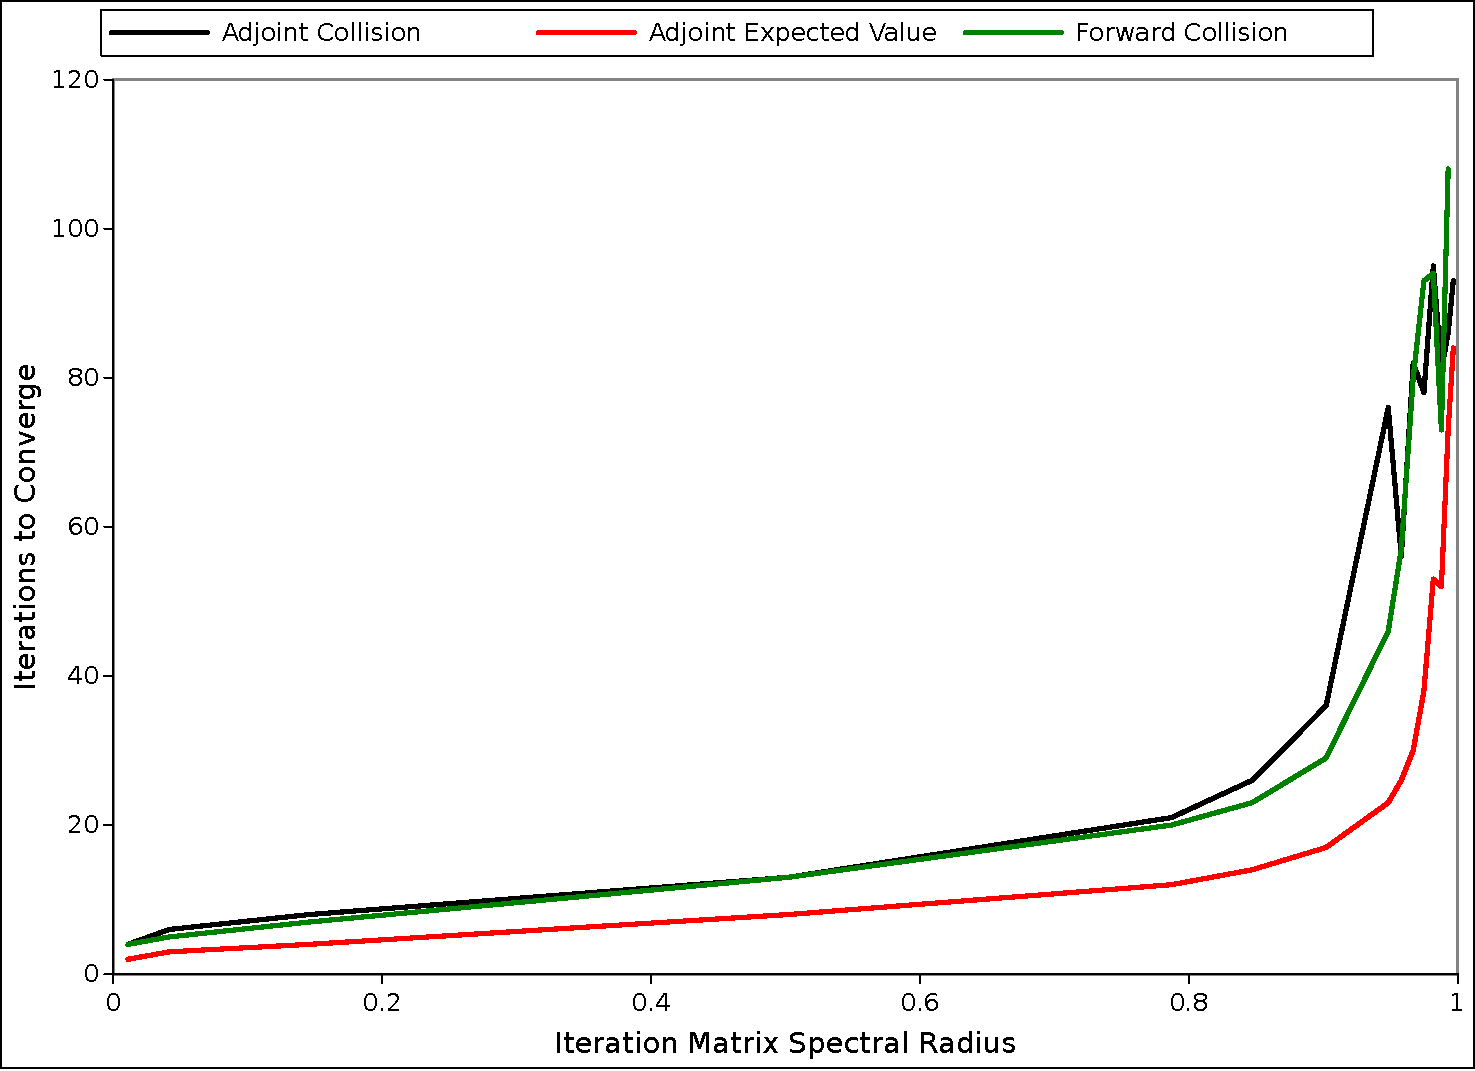
\includegraphics[width=5in]{chapters/spn_equations/breakdown_iterations.pdf}
  \end{center}
  \caption{\textbf{Iterations required to converge as a function of
      spectral radius for the neutron diffusion problem.} \textit{The
      number of histories was increased to achieve convergence in less
      than 100 iterations. At least 10,000 histories were used for
      each calculation.}}
  \label{fig:breakdown_iterations}
\end{figure}
\begin{figure}[t!]
  \begin{center}
    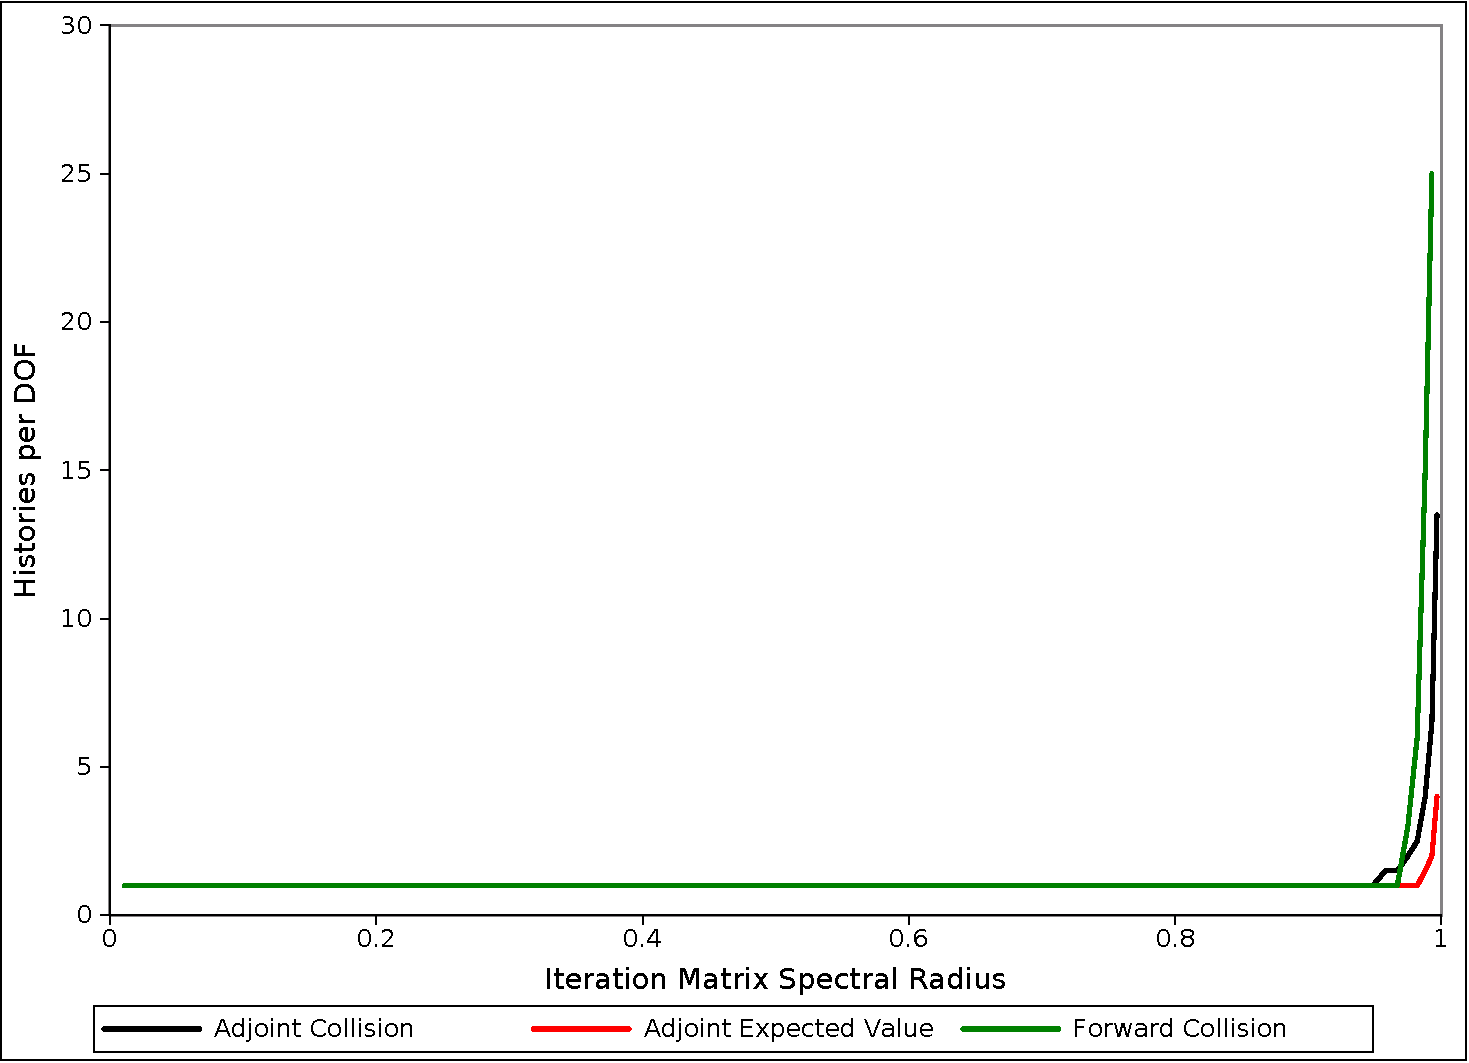
\includegraphics[width=5in]{chapters/spn_equations/breakdown_histories.pdf}
  \end{center}
  \caption{\textbf{Histories required to converge as a function of
      spectral radius for the neutron diffusion problem.} \textit{The
      number of histories was increased to achieve convergence in less
      than 100 iterations. At least 10,000 histories were used for
      each calculation.}}
  \label{fig:breakdown_histories}
\end{figure}
In addition to the significantly larger number of histories required
for to achieve convergence for ill-conditioned problems another
penalty is paid due to histories that take longer to
compute. Figure~\ref{fig:breakdown_time} gives the CPU time in
seconds required to compute a single random walk averaged over the
entire set of histories run in the calculation over all iterations. As
the spectral radius increases (correlating to a higher ratio of
scattering in the system) the random walk lengths increase, using more
CPU time to finish the computation. Compared to spectral radii of 0.5,
larger spectral radii over 0.97 have histories that require two orders
of magnitude more computation time. This signficant increase in
computation time per history coupled with the significant increase in
the number of histories required to converge is evidence that for
problems with spectral radii above $\approx 0.97$, using MCSA to solve
any problems of interest is completely intractable. We therefore
require a more expansive set of preconditioning techniques to reduce
the eigenvalue spectrum of the $SP_N$ problem into a regime in which
MCSA is more applicable.
\begin{figure}[t!]
  \begin{center}
    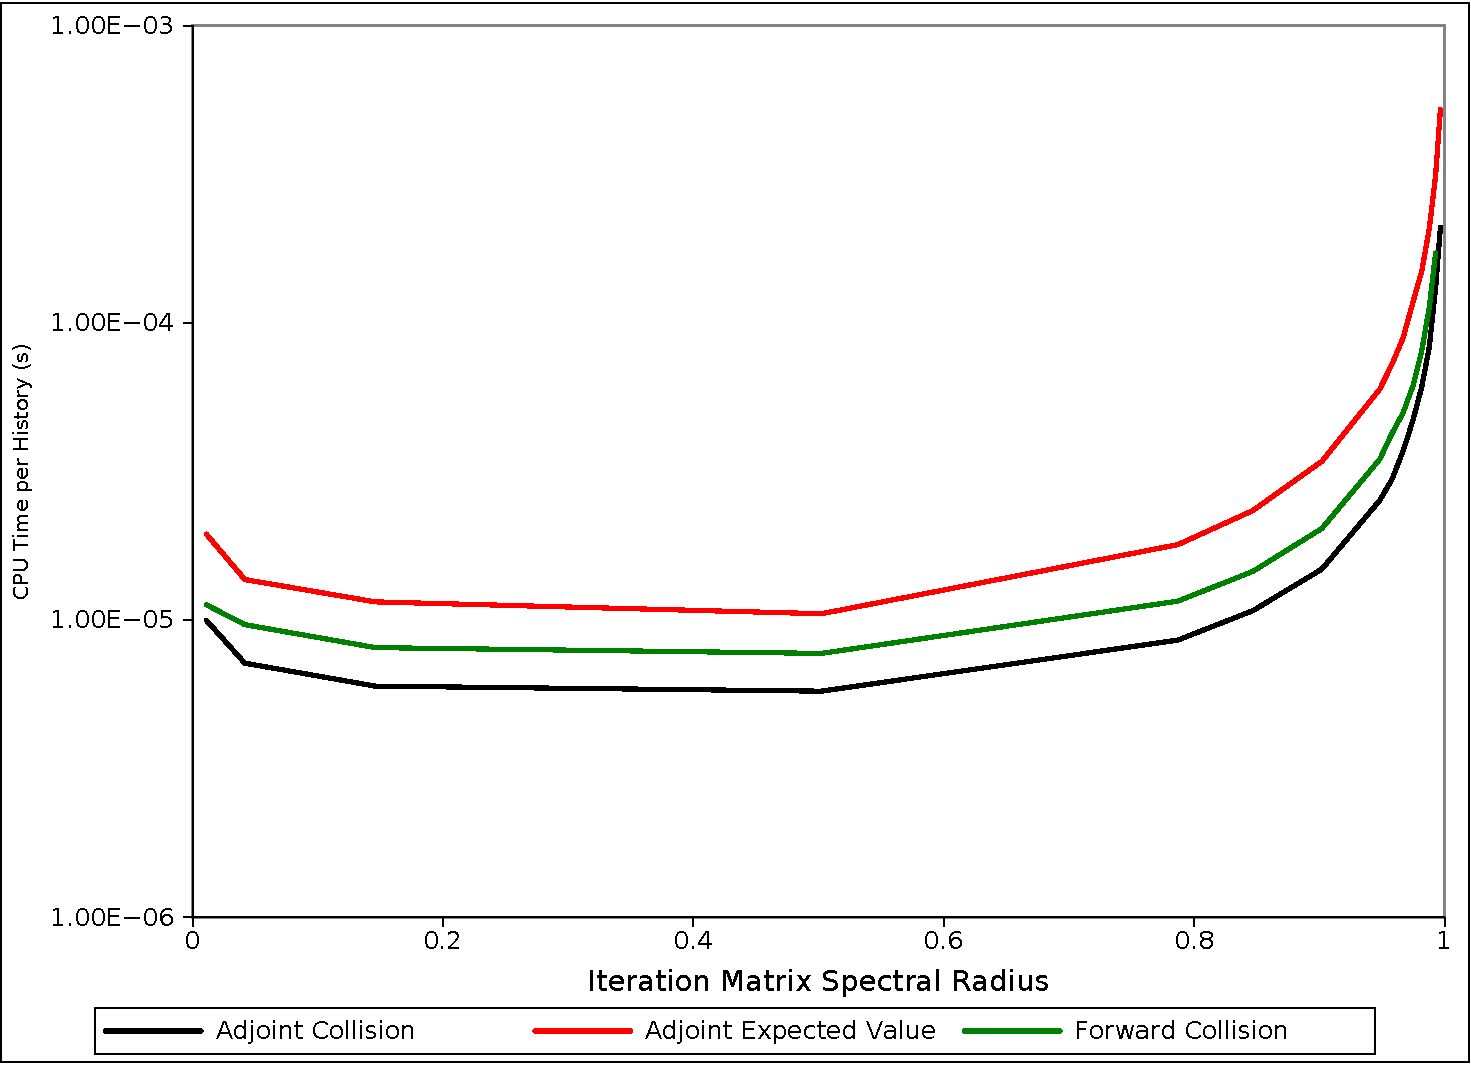
\includegraphics[width=5in]{chapters/spn_equations/breakdown_time.pdf}
  \end{center}
  \caption{\textbf{CPU time per history as a function of spectral
      radius for the neutron diffusion problem.} \textit{As the
      spectral radius grows, so do the length of the random
      walks. Longer random walks require more CPU time to compute.}}
  \label{fig:breakdown_time}
\end{figure}

\clearpage

%%---------------------------------------------------------------------------%%
\section{Advanced Preconditioning Strategies}
\label{subsec:spn_advanced_preconditioning}

\subsection{ILUT Preconditioning}
\label{subsec:spn_ilut_preconditioning}

\subsection{Sparse Approximate Inverse Preconditioning}
\label{subsec:spn_spainv_preconditioning}

\subsection{SPAINV Improved ILUT Preconditioning}
\label{subsec:spn_spainv_preconditioning}

\subsection{MCSA Relaxation Parameters}
\label{subsec:spn_mcsa_relaxation}

\subsection{Monte Carlo Estimator Comparison}
\label{subsec:spn_estimator_comparison}

%%---------------------------------------------------------------------------%%
\section{MCSA Comparison to Conventional Methods}
\label{sec:spn_comparison}

